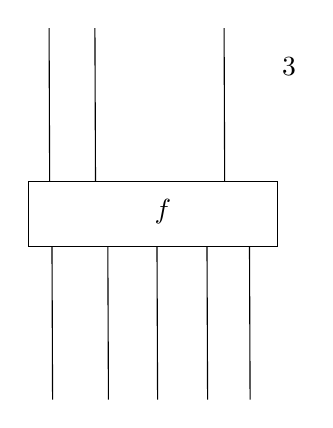
\begin{tikzpicture}[yscale=-1,scale=0.1,baseline={([yshift=-.5ex]current bounding box.center)}]
\begin{scope}[shift={(0.00mm,203.00mm)}]
\draw [fill=none,draw=black] (18.89mm,-3.12mm) rectangle (335.46mm,79.29mm) ;
% path id='path12'
% path spec='M 46.113094,-3.8690455 45.357142,-198.14881'
\draw [fill=none,draw=black] (46.11mm,-3.87mm)
-- (45.36mm,-198.15mm)
;
% path id='path14'
% path spec='M 104.32143,-3.8690455 103.56548,-198.14881'
\draw [fill=none,draw=black] (104.32mm,-3.87mm)
-- (103.57mm,-198.15mm)
;
% path id='path16'
% path spec='M 268.36284,-3.8690455 267.60689,-198.14881'
\draw [fill=none,draw=black] (268.36mm,-3.87mm)
-- (267.61mm,-198.15mm)
;
% path id='path18'
% path spec='M 300.64221,273.3766 299.88626,79.096795'
\draw [fill=none,draw=black] (300.64mm,273.38mm)
-- (299.89mm,79.10mm)
;
% path id='path20'
% path spec='M 246.66711,273.3766 245.91116,79.096795'
\draw [fill=none,draw=black] (246.67mm,273.38mm)
-- (245.91mm,79.10mm)
;
% path id='path22'
% path spec='M 183.16707,273.3766 182.41112,79.096795'
\draw [fill=none,draw=black] (183.17mm,273.38mm)
-- (182.41mm,79.10mm)
;
% path id='path24'
% path spec='M 120.72525,273.3766 119.9693,79.096795'
\draw [fill=none,draw=black] (120.73mm,273.38mm)
-- (119.97mm,79.10mm)
;
% path id='path26'
% path spec='M 49.817166,273.3766 49.061216,79.096795'
\draw [fill=none,draw=black] (49.82mm,273.38mm)
-- (49.06mm,79.10mm)
;

\node at (190mm,35mm) {$f$};
\node at (350mm,-150mm) {$\ydiagram{3}$};

\end{scope}
\end{tikzpicture}
